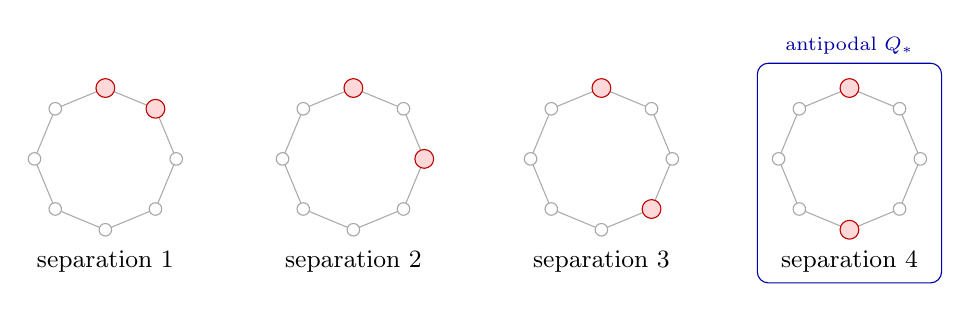
\begin{tikzpicture}[scale=.9,
 dot/.style={circle,draw=gray!70,fill=white,inner sep=1.6pt},
 defect/.style={circle,draw=red!75!black,fill=red!15,inner sep=2.4pt}]
\foreach \sep/\x/\lab in {1/0/$1$,2/3.5/$2$,3/7/$3$,4/10.5/$4$}{
  \begin{scope}[xshift=\x cm]
    \draw[gray!65] (0:1)--(45:1)--(90:1)--(135:1)--(180:1)--(225:1)--(270:1)--(315:1)--cycle;
    \foreach \j in {0,...,7}{\node[dot] (n\sep-\j) at ({90-45*\j}:1) {};}
    \node[defect] at (n\sep-0) {};
    \node[defect] at (n\sep-\sep) {};
    \node[font=\small] at (0,-1.45) {separation \lab};
    \ifnum\sep=4
      \draw[blue!65!black,rounded corners] (-1.3,-1.75) rectangle (1.3,1.35);
      \node[blue!65!black,font=\scriptsize] at (0,1.6) {antipodal $Q_*$};
    \fi
  \end{scope}
}
\end{tikzpicture}
